\subsection{Máquinas de vetores de suporte}

Para implementar a técnica de máquinas de vetores de suporte utilizamos a conhecida biblioteca LIBSVM \cite{libsvm} e também uma breve leitura inicial de um guia \cite{libsvm_guide}, disponibilizado pelos principais responsáveis pela biblioteca.

Seguindo as recomendações providas pelo guia, iniciamos alguns testes com a função \emph{kernel} Gaussiana (\emph{Radial Basis Function}), dada por:

\begin{equation}
	K(x, y) = e^{-\gamma ||x - y||^2}
\end{equation}

Portanto, temos 2 hiperparâmetros a serem escolhidos, $C$ e $\gamma$. Sendo $C$ o parâmetro de penalização, ou seja, é o \emph{trade-off} entre classificar uma amostra de treino erroneamente contra a simplificação da superfície de decisão. Um valor baixo resulta em uma fronteira de decisão suave, e quanto maior o valor, maior a tendência de classificar todas as amostras de treino corretamente, dando ao modelo plena liberdade de escolher mais amostras como vetores de suporte.

Já o parâmetro $\gamma$ define qual o alcance de influência de uma única amostra de treino, onde um valor baixo indica longo alcance e um valor alto indica curto alcance. Este parâmetro pode ser visto como o inverso do raio de influência das amostras selecionadas pelo modelo como vetores de suporte. É possível observar, de forma mais intuitiva e visual o comportamento destes parâmetros na Figura \ref{fig:grafico_rbf_demo}.

\begin{figure}[ht]
  \centering
    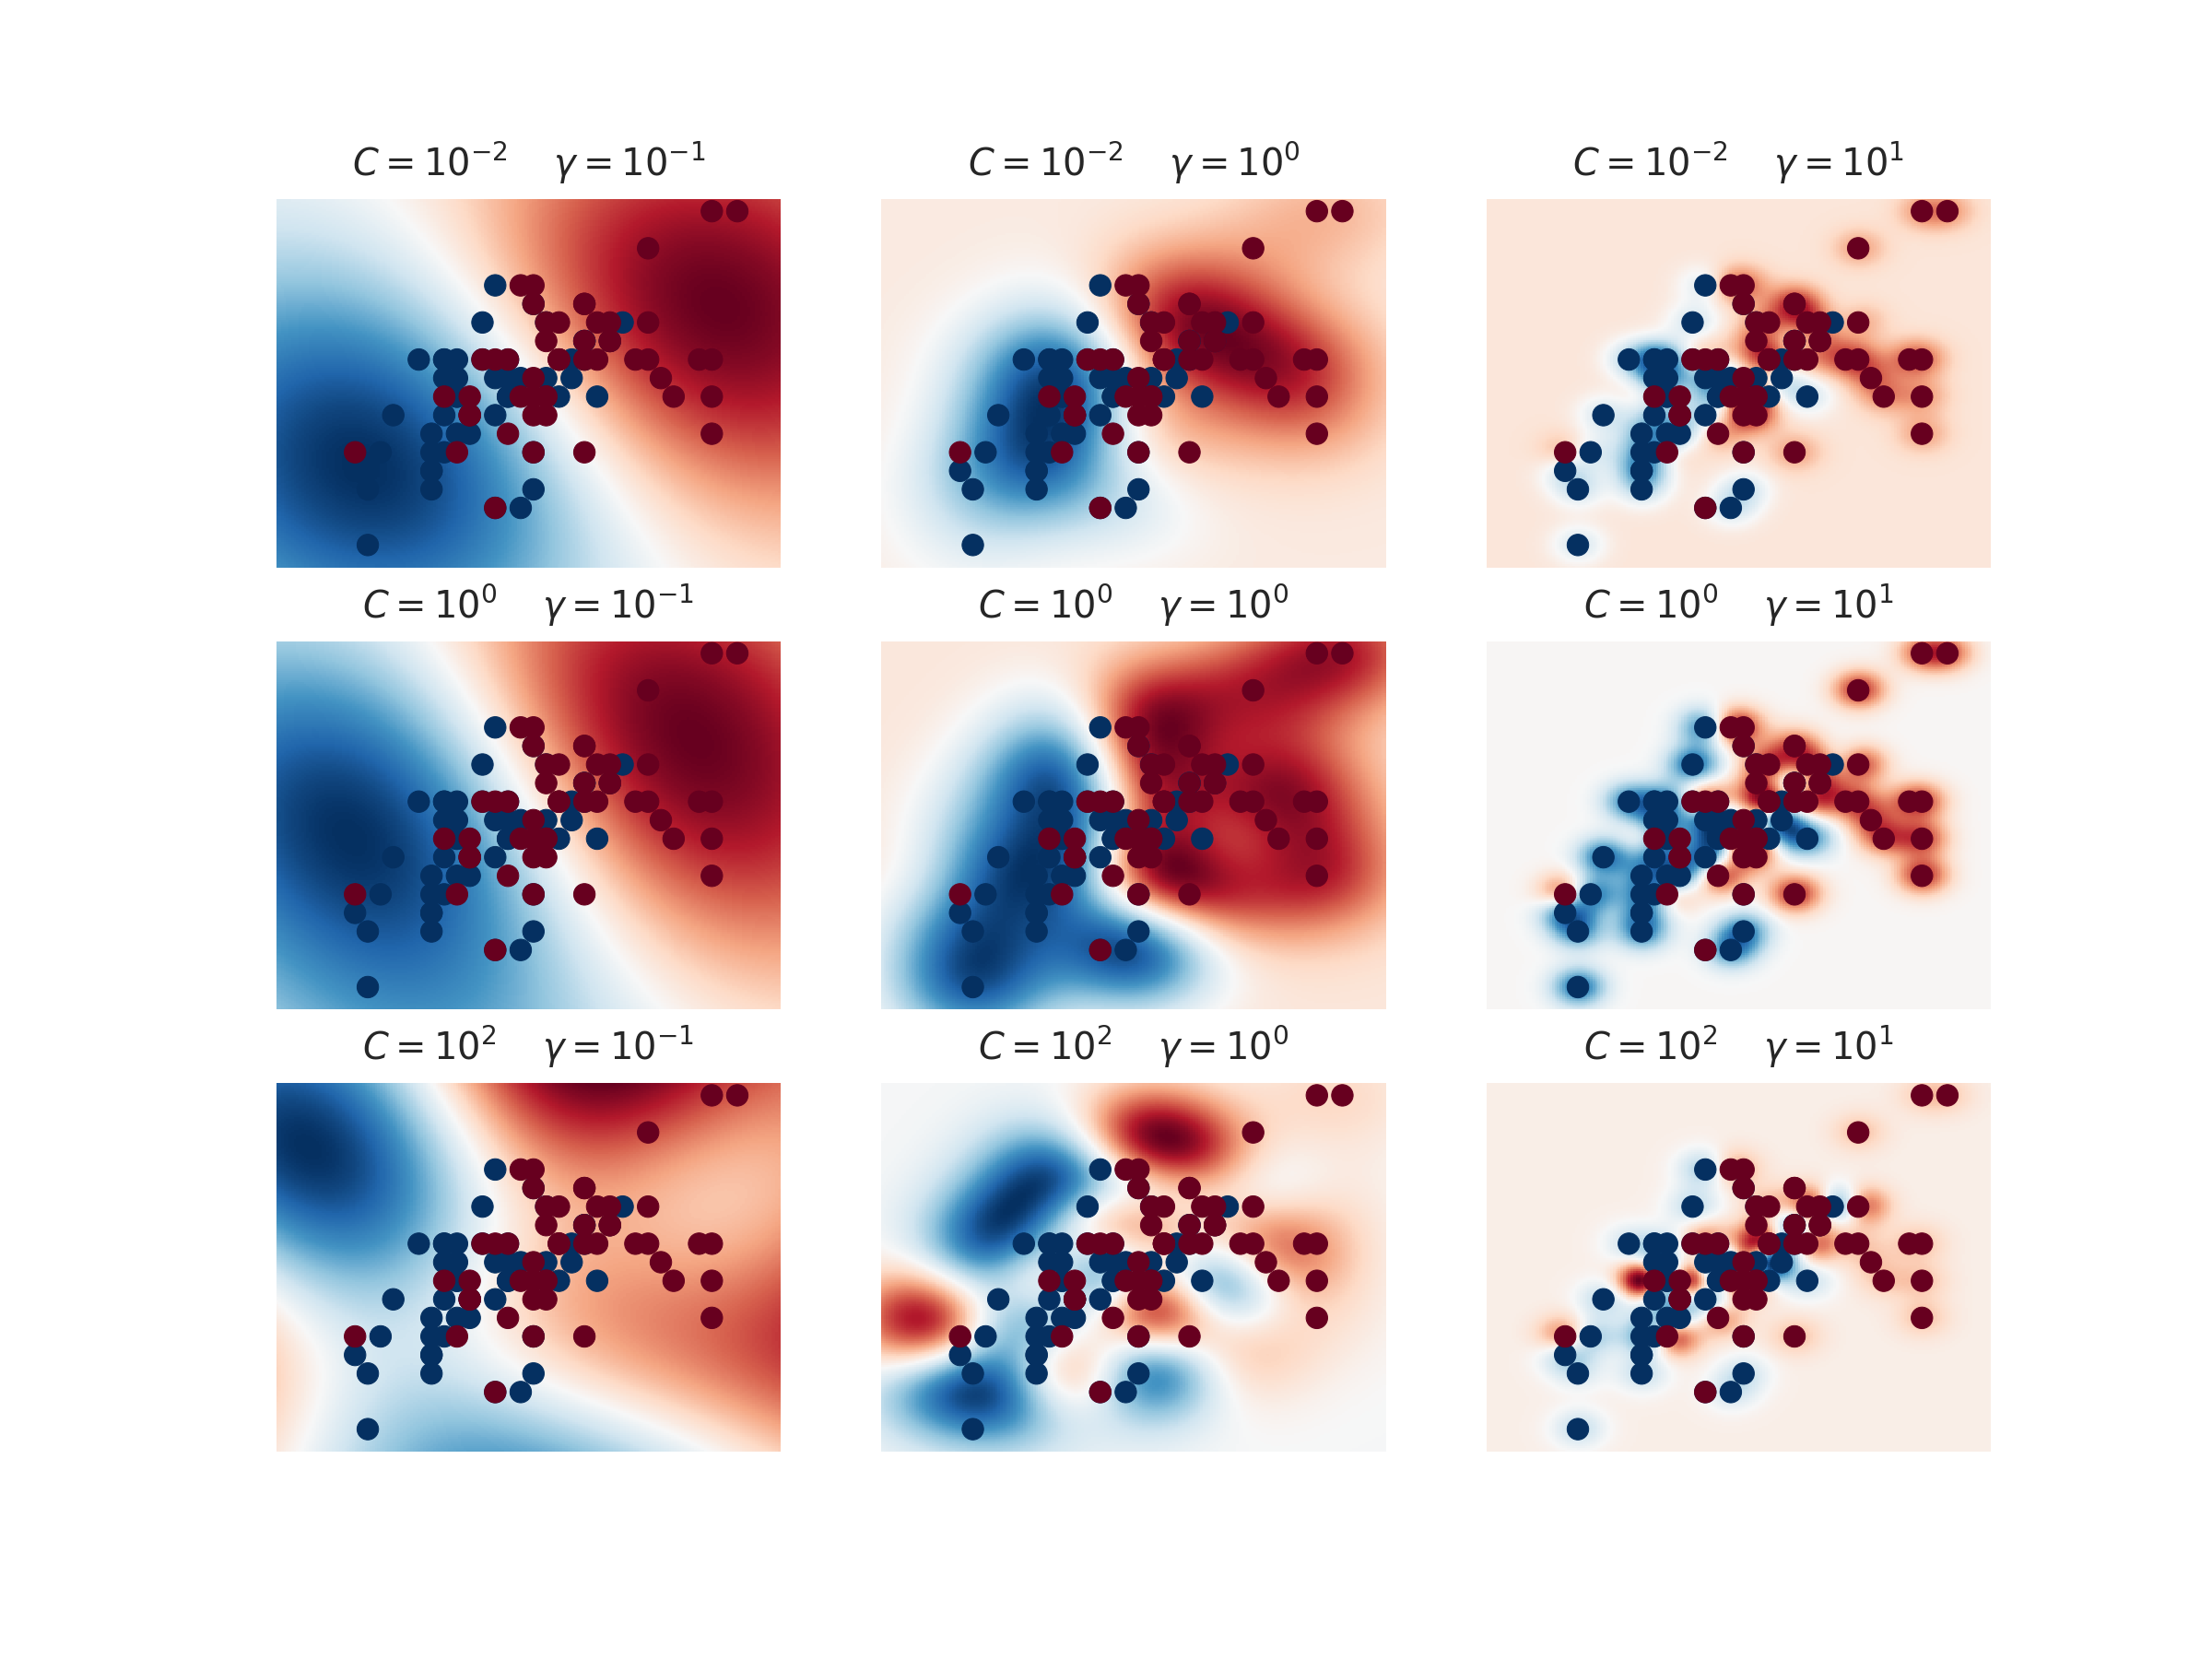
\includegraphics[width=0.5\textwidth]{rbf_hyperparams_demo.png}
    \caption{Demonstração do comportamento de $C$ e $\gamma$ utilizando como exemplo o \emph{Iris Dataset} \cite{uci_ml_repo}}
    \label{fig:grafico_rbf_demo}
\end{figure}

Após termos escolhido inicialmente o \emph{kernel} RBF para os primeiros testes, uma leitura mais a fundo mostrou também os seguintes pontos importantes que nos levaram a escolha definitiva desta função \emph{kernel}.

O \emph{kernel} RBF mapeia as amostras de forma não linear para um espaço dimensional maior, portanto, pode lidar com casos onde a relação entre os atributos e a classe não são lineares. Além do mais, ele possui a mesma performance de um \emph{kernel} linear com parâmetro de penalização $\tilde{C}$  \cite{rbf_linear}.

Outro fato muito importante é o número de hiperparâmetros a serem escolhidos, os quais influenciam a complexidade de seleção do modelo. O \emph{kernel} polinomial é dado por:

\begin{equation}
	K(x, y) = (\gamma x^T y + r)^d
\end{equation}

Ou seja, temos quatro hiperparâmetros para serem selecionados: $C$, $\gamma$, $r$ e $d$. Além disso, o \emph{kernel} polinomial pode sofrer com dificuldades numéricas, onde os valores do \emph{kernel} podem tender a infinito $(\gamma x^T y + r > 1)$ ou zero $(\gamma x^T y + r < 0)$ quando o grau($d$) é alto, enquanto os valores do \emph{kernel} RBF ficam entre 0 e 1 $(0 < K_{ij} < 1)$.

Para otimizarmos os hiperparâmetros $C$ e $\gamma$ realizamos busca em \emph{grid} com \emph{5-fold cross-validation}. Segundo o guia, sequências que crescem exponencialmente são um método prático para se identificar bons parâmetros \cite{libsvm_guide}. Portanto, seguindo as recomendações do mesmo, optamos por realizar duas buscas em \emph{grid}. Ambas as buscas foram realizadas duas vezes, sendo uma aplicando PCA e outra não, e ambas com normalização dos atributos.

A primeira busca possui um intervalo mais amplo entre os valores exponenciais, sendo seu \emph{step} de $2^2$ e as seguintes sequências: $C = 2^{-5}, 2^{-3}, ..., 2^{15}$ e $\gamma = 2^{-13}, 2^{-11}, ..., 2^1$. Após realizada a primeira busca agrupamos todos os resultados por cada parâmetro e tiramos a média e desvio padrão da acurácia e MCC para identificamos os intervalos de $C$ e $\gamma$ que obtiveram os melhores resultados, como podemos obserar na Tabela \ref{tab:svm_coarse_grid_table}.

\begin{table}[ht]
\centering
\begin{tabular}{@{}lcc|ccr@{}}
\toprule
\multirow{2}{*}{} & \multicolumn{2}{c|}{$C$}                   & \multicolumn{2}{c}{$\gamma$} & \multicolumn{1}{l}{\multirow{2}{*}{}} \\ \cmidrule(lr){2-5}
                  & Acc       & MCC                        & Acc       & MCC           & \multicolumn{1}{l}{}                  \\ \midrule
$2^{-5}$          & $0.65 \pm 0.14$ & $0.32 \pm 0.28$              & $0.80 \pm 0.12$ & $0.60 \pm 0.23$ & $2^{-13}$                             \\
$2^{-3}$          & $0.73 \pm 0.13$ & $0.49 \pm 0.24$              & $0.84 \pm 0.06$ & $0.68 \pm 0.12$ & $2^{-11}$                             \\
$2^{-1}$          & $0.79 \pm 0.09$ & $0.60 \pm 0.15$              & $\bf{0.85 \pm 0.04}$ & $\bf{0.70 \pm 0.08}$ & $2^{-9}$                              \\
$2^{1}$           & $\bf{0.82 \pm 0.06}$ & $\bf{0.66 \pm 0.10}$              & $\bf{0.85 \pm 0.03}$ & $\bf{0.70 \pm 0.05}$ & $2^{-7}$                              \\
$2^{3}$           & $\bf{0.83 \pm 0.06}$ & $\bf{0.66 \pm 0.11}$              & $\bf{0.84 \pm 0.03}$ & $\bf{0.68 \pm 0.05}$ & $2^{-5}$                              \\
$2^{5}$           & $\bf{0.83 \pm 0.06}$  & $\bf{0.66 \pm 0.11}$              & $0.81 \pm 0.04$ & $0.62 \pm 0.06$ & $2^{-3}$                              \\
$2^{7}$           & $0.82 \pm 0.06$ & $0.65 \pm 0.11$              & $0.72 \pm 0.09$ & $0.47 \pm 0.18$ & $2^{-1}$                              \\
$2^{9}$           & $0.82 \pm 0.06$ & $0.65 \pm 0.11$              & $0.65 \pm 0.09$ & $0.34 \pm 0.19$ & $2^{1}$                              \\
$2^{11}$          & $0.82 \pm 0.06$ & $0.64 \pm 0.11$              &       -        &        -       & \multicolumn{1}{c}{-}                 \\
$2^{13}$          & $0.81 \pm 0.06$ & $0.63 \pm 0.11$ &  -             &       -        & \multicolumn{1}{c}{-}                 \\ \bottomrule
\end{tabular}
\caption{Resultados do \emph{Coarse Grid Search} sem PCA}
\label{tab:svm_coarse_grid_table}
\end{table}

Apesar da sequência que definimos inicialmente para $C$ ir até $2^{15}$ não chegamos a concluir a busca em \emph{grid} neste último exponencial devido ao alto custo computacional, exigindo um grande número de iterações pela SVM e demorando consideravelmente em cada \emph{fold} da validação cruzada, além disso, tanto a acurácia quanto o MCC já se encontravam em queda a partir do exponencial $2^7$.

A segunda busca possui um intervalo mais curto entre os valores exponenciais, sendo seu step de $2^{0.25}$ e as sequências obtidas a partir da primeira busca foram: $C = 2^{1}, 2^{1.25}, ..., 2^{5}$ e $\gamma = 2^{-9}, 2^{-9.25}, ..., 2^{-5}$, como pudemos observar na Tabela \ref{tab:svm_coarse_grid_table}.

Feita essa busca em \emph{grid} mais fina, selecionamos $C = 2^{4.25}$ e $\gamma = 2^{-7.25}$ sem PCA, como os hiperparâmetros ótimos.